\documentclass{chi-ext}
% Please be sure that you have the dependencies (i.e., additional LaTeX packages) to compile this example.
% See http://personales.upv.es/luileito/chiext/

\copyrightinfo{
  Copyright is held by the author/owner(s).\\
  \emph{MOBILEHCI'14}, April 27 -- May 2, 2013, Toronto, Canada.\\
  ACM 978-1-XXXX-XXXX-X/XX/XX.\\
}

\title{Low resolution wearable vibrotactile displays.}

\numberofauthors{5}
% Notice how author names are alternately typesetted to appear ordered in 2-column format;
% i.e., the first 4 autors on the first column and the other 4 auhors on the second column.
% Actually, it's up to you to strictly adhere to this author notation.
\author{
  \alignauthor{
  	\textbf{Adam Tindale}\\
  	\affaddr{OCAD University}\\
  	\affaddr{Toronto, ON M5T 1W1 Canada}\\
  	\email{atindale@faculty.ocadu.ca}
  }\alignauthor{
  	\textbf{Michael Cumming}\\
  	\affaddr{OCAD University}\\
  	\affaddr{Toronto, ON M5T 1W1 Canada}\\
  	\email{mcumming@ocadu.ca}
  }\alignauthor{
  	\textbf{Huson Pridham}\\
  	\affaddr{OCAD University}\\
  	\affaddr{Toronto, ON M5T 1W1 Canada}\\
  	\email{hp12pk@student.ocadu.ca}
  }\alignauthor{
  	\textbf{Jessica Peter}\\
  	\affaddr{OCAD University}\\
  	\affaddr{Toronto, ON M5T 1W1 Canada}\\
  	\email{jp11jg@student.ocadu.ca}
  }\alignauthor{
  	\textbf{Sara Diamond}\\
  	\affaddr{OCAD University}\\
  	\affaddr{Toronto, ON M5T 1W1 Canada}\\
  	\email{sdiamond@ocadu.ca}
  }
}

\teaser{
  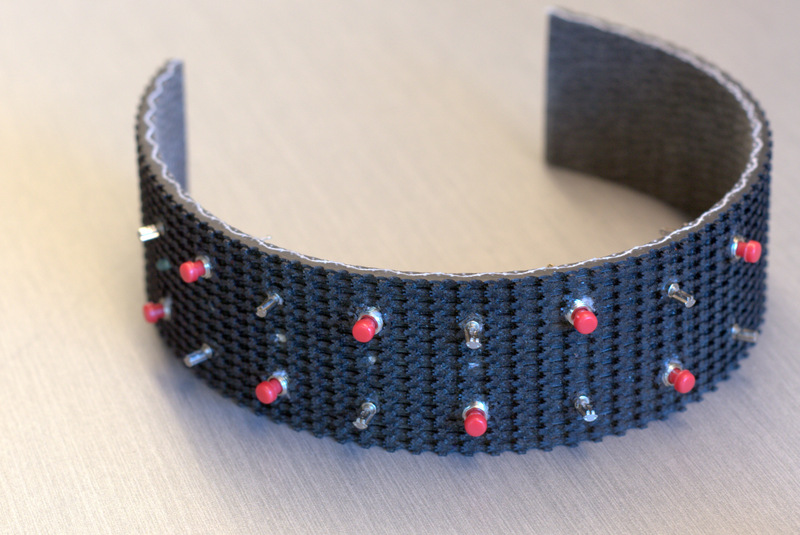
\includegraphics[width=\columnwidth]{images/P1130383.jpg}
  \caption{First prototype of a wrist based multi-channel vibrotactile display..}
  \label{fig:vibrobelt1}
}

% Paper metadata (use plain text, for PDF inclusion and later re-using, if desired)
\def\plaintitle{CHI LaTeX Extended Abstracts Template}
\def\plainauthor{Adam Tindale}
\def\plainkeywords{Guides, instructions, author's kit, conference publications}
\def\plaingeneralterms{Documentation, Standardization}

\hypersetup{
  % Your metadata go here
  pdftitle={\plaintitle},
  pdfauthor={\plainauthor},  
  pdfkeywords={\plainkeywords},
  pdfsubject={\plaingeneralterms},
  % Quick access to color overriding:
  citecolor=black,
  linkcolor=blue,
  menucolor=black,
  urlcolor=blue,
}

\usepackage{graphicx}   % for EPS use the graphics package instead
\usepackage{balance}    % useful for balancing the last columns
\usepackage{bibspacing} % save vertical space in references



\begin{document}

\maketitle

\begin{abstract}
In this paper we describe a series of demo experiences focusing on the communication of information through low resolution vibractile and LED displays.
\end{abstract}

\keywords{\plainkeywords}
\textcolor{red}{Mandatory section to be included in your final version.}

\category{H.5.m}{Information interfaces and presentation (e.g., HCI)}{Miscellaneous}. 
%See \cite{ACMCCS} 
See: \url{http://www.acm.org/about/class/1998/} 
\textcolor{red}{Mandatory section to be included in your final version.}

\terms{\plaingeneralterms}
\textcolor{red}{Optional section to be included in your final version.}


% =============================================================================
\section{Introduction}
% =============================================================================


% =============================================================================
\section{Background}
% =============================================================================


% =============================================================================
\section{Text formatting}
% =============================================================================
Please use an 8.5-point Verdana font, or other sans serifs font as close as possible in appearance to Verdana in which these guidelines have been set. 
Arial 9-point font is a reasonable substitute for Verdana as it has a similar x-height. 
Please use serif or non-proportional fonts only for special purposes, such as distinguishing source code text.
Additionally, here is an example of footnoted text.\footnote{Use footnotes sparingly, if at all.}
As stated in the footnote, footnotes should rarely be used.

\subsection{Language, style, and content}
% -----------------------------------------------------------------------------
The written and spoken language of SIGCHI is English. 
Spelling and punctuation may use any dialect of English (e.g., British, Canadian, US, etc.) provided this is done consistently. 
Hyphenation is optional. 
To ensure suitability for an international audience, please pay attention to the following:

\begin{itemize}\compresslist
\item 	
Write in a straightforward style. 
Use simple sentence structure. 
Try to avoid long sentences and complex sentence structures. 
Use semicolons carefully.
\item 	
Use common and basic vocabulary (e.g., use the word ``unusual" rather than the word ``arcane").
\item 	
Briefly define or explain all technical terms. 
The terminology common to your practice/discipline may be different in other design practices/disciplines.
\item 	
Spell out all acronyms the first time they are used in your text. 
For example, ``World Wide Web (WWW)".
\item 	
Explain local references (e.g., not everyone knows all city names in a particular country).
\item 	
Explain ``insider" comments. 
Ensure that your whole audience understands any reference whose meaning you do not describe (e.g., do not assume that everyone has used a Macintosh or a particular application).
\item 	
Explain colloquial language and puns. 
Understanding phrases like ``red herring" requires a cultural knowledge of English. 
Humor and irony are difficult to translate.
\item 	
Use unambiguous forms for culturally localized concepts, such as times, dates, currencies and numbers (e.g., ``1-5-97" or ``5/1/97" may mean 5 January or 1 May, and ``seven o'clock" may mean 7:00 am or 19:00).
\item 	
Be careful with the use of gender-specific pronouns (he, she) and other gender-specific words (chairman, manpower, man-months). 
Use inclusive language (e.g., she or he, they, chair, staff, staff-hours, person-years) that is gender-neutral. 
If necessary, you may be able to use ``he" and ``she" in alternating sentences, so that the two genders occur equally often~\cite{Schwartz95}. 
\end{itemize}


% =============================================================================
\section{Figures}
% =============================================================================

Your document may use color figures, which are included in the page limit; the figures must be usable when printed in black and white.
You can use the \LaTeX's \texttt{marginpar} command to insert figures in the (right) margin side of the document (see \autoref{fig:marginparsample}).

As shown in \autoref{fig:sample}, the width of figures can be bigger than the width of text columns.
\autoref{fig:bigsample} is an example of how much space can be reserved for images.


% =============================================================================
\section{References and Citations}
% =============================================================================
Use a numbered list of references at the end of the article, ordered alphabetically by first author, and referenced by numbers in brackets \cite{Anderson92,Klemmer02,Mather00,Zellweger01}
For papers from conference proceedings, include the title of the paper and an abbreviated name of the conference (e.g., for Interact 2003 proceedings, use Proc. Interact 2003). 
Do not include the location of the conference or the exact date; do include the page numbers if available. 
See the examples of citations at the end of this document. 

Your references should be published materials accessible to the public.  
Internal technical reports may be cited only if they are easily accessible (i.e., you provide the address for obtaining the report within your citation) and may be obtained by any reader for a nominal fee.  
Proprietary information may not be cited. 
Private communications should be acknowledged in the main text, not referenced  (e.g., [Robertson, personal communication]).


% =============================================================================
\section{Felted Wearable}
% =============================================================================
\marginpar{
\begin{figure}
  \begin{center}
  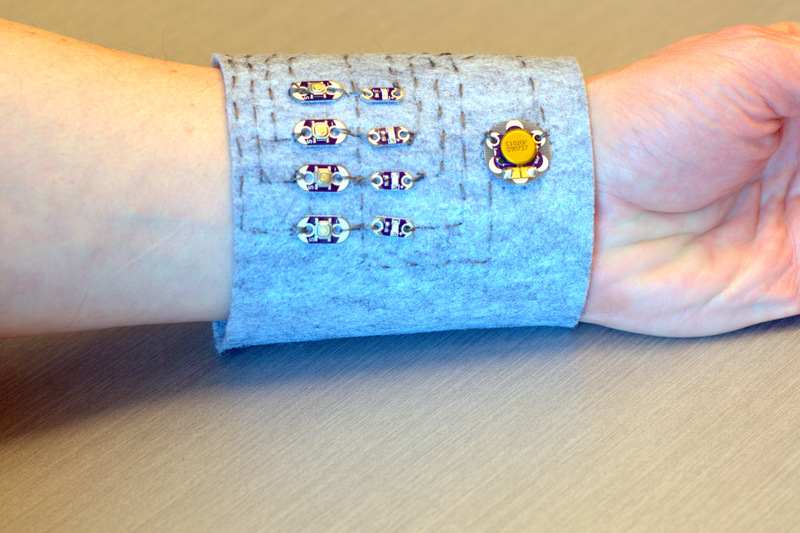
\includegraphics[width=\marginparwidth]{images/P1130375.jpg}
  \caption{A wearable interface.}
  \label{fig:marginparsample}
  \end{center}  
\end{figure}
}


\section{Acknowledgements}
We thank all the volunteers, and all publications support and staff, who wrote and provided helpful comments on previous versions of this document. This work is generously supported by the Natural Sciences and Engineering Research Council of Canada (NSERC), International Science and Technology Partnerships Canada.

\balance
\bibliographystyle{acm-sigchi}
\bibliography{sample}

\end{document}
